\documentclass[conference]{IEEEtran}
\IEEEoverridecommandlockouts
% The preceding line is only needed to identify funding in the first footnote. If that is unneeded, please comment it out.
\usepackage{cite}
\usepackage{amsmath,amssymb,amsfonts}
\usepackage{algorithmic}
\usepackage{graphicx}
\usepackage{textcomp}
\usepackage[x11names]{xcolor}
\usepackage{gensymb}
\usepackage{wasysym}
\usepackage{graphics}
\usepackage{bm}
\usepackage{xfrac}
\usepackage{siunitx}
\usepackage{pgfplots}
\usepackage{tikz, tikz-3dplot}
\usepackage{xfp}
\usepackage{dutchcal}
\usepackage{float}
\def\BibTeX{{\rm B\kern-.05em{\sc i\kern-.025em b}\kern-.08em
	T\kern-.1667em\lower.7ex\hbox{E}\kern-.125emX}}
\graphicspath{ {./html/} }
\makeatletter
\newcommand*{\overrightharpoonup}{\mathpalette{\overarrow@\rightharpoonupfill@}}
\newcommand*{\rightharpoonupfill@}{\arrowfill@\relbar\relbar\rightharpoonup}
\makeatother
\renewcommand{\vec}[1]{\overrightharpoonup{\bm{\mathrm{#1}}}}
\newcommand{\vhat}[1]{\hat{\bm{\mathrm{#1}}}}
\newcommand{\abs}[1]{\lvert#1\rvert}
\newcommand{\norm}[1]{\abs{\abs{\vec{#1}}}}

\begin{document}

	\sisetup{per-mode = fraction, fraction-function = \sfrac}
	\sisetup{exponent-product = \ensuremath { { } \cdot { } } }

	\title{Two-Line Element Decoder and Visualizer\\
		{\footnotesize UNM ECE 535 Final Project: Software Type}
	}

	\author{\IEEEauthorblockN{Sonny Ji}
		\IEEEauthorblockA{\textit{Department of Electrical and Computer Engineering} \\
		\textit{The University of New Mexico}\\
		Albuquerque, United States \\
		velten@unm.edu}
	}

	\maketitle

	\begin{abstract}
		This document details the conceptualization, design, implementation, and finalization of a software tool for visualizing the orbits of satellites. The goal of this tool is to aid in the visualization of satellites and their orbits, along with a presentation that promotes a human-digestible format for better intuition and understanding of satellite orbital mechanics and satellite communication ranges.
	\end{abstract}

	\begin{IEEEkeywords}
		satellite communications, TLE, orbital mechanics, 3D-simulation, software
	\end{IEEEkeywords}

	\section{Introduction}
		This is a project for the ECE 535 Satellite Communications class at The University of New Mexico's Department of Electrical and Computer Engineering. The goal of this project is to develop and build a desktop application for decoding two-line element sets and representing the results in an interactive 3D graphic that tracks the satellite. Additionally, this tool will attempt to further append satellite information through pinging web-based APIs for further satellite information and data. This would include items (when applicable) such as: orbit lines, satellite use and type, cone of coverage, trajectory, Earth for scale, and visualizations of all 6 classical orbital mechanics parameters. The deliverable for this project is an application / software package for taking in two-line element sets as an input and presenting 3D models of the previously described as an output, along with a brief guide on how to use and interpret the tool.

		Information on the tool and a guide on how to use it are included at the end of this document under the \textit{Usage Information and Notes} section.

	\section{Useful Information and Definitions}

		\subsection{Abbreviations and Acronyms}\label{AA}
			\begin{itemize}
				\item TLE: Two-Line Element
				\item AN: Ascending Node
				\item DN: Descending Node
				\item RAAN: Right Ascension of the Ascending Node
			\end{itemize}

		\subsection{Variables and Symbols}
			\begin{itemize}
				\item \( a \): Semi-major axis of elliptical orbit
				\item \( b \): Semi-minor axis of elliptical orbit
				\item \( e \): Eccentricity of elliptical orbit
				\item \( i \): Inclination of elliptical orbit
				\item \( \Omega \): RAAN, longitude of the ascending node
				\item \( \omega \): Argument of periapsis of elliptical orbit
				\item \( \nu \): True anomaly of elliptical orbit
				\item \( \aries \): First point of Aries, vernal equinox
				\item \( \ascnode \): AN
				\item \( \descnode \): DN
				\item \( M \): Mean anomaly of elliptical orbit
				\item \( E \): Elliptical anomaly of elliptical orbit
				\item \( n \): Mean motion of elliptical orbit
				\item \( R \): Radius of celestial body
				\item \( r \): Radius of orbit with respect to central orbiting body
			\end{itemize}

		\subsection{Subscripts}
			\begin{itemize}
				\item \( \cdot_a \): Relating to the apoapsis of an orbit
				\item \( \cdot_p \): Relating to the periapsis of an orbit
				\item \( \cdot_{\oplus} \): Relating to the Earth
				\item \( \cdot_0 \): Relating to epoch
			\end{itemize}

		\subsection{Units}
			\begin{itemize}
				\item All distances (i.e. \( a \), \( r_p \), \( R_{\oplus} \), etc.) are presented in kilometers
				\item All velocities (i.e. \( v_p \), \( v_a \), \( \vec{v} \), etc.) are presented in kilometers per second
				\item All angles (i.e. \( \nu_0 \), \( E_0 \), \( M_0 \), etc.) are presented in radians
				\item All angular velocities (i.e. \( \omega_{\oplus} \), \( n \), etc.) are presented in radians per second
				\item All durations (i.e. \( \Delta t \), etc.) are presented in seconds
			\end{itemize}

		\subsection{Constants}
			\begin{itemize}
				\item \( R_{\oplus}=\qty{6378}{\kilo\meter} \)
				\item \( \omega_{\oplus}=\qty{7.2921159e-5}{\radian\per\second} \)
				\item \( \mu_{\oplus}=\qty{3.986e5}{{\kilo\meter^3}\per{\second^2}} \)
			\end{itemize}

	\section{Motivations and Methodologies}

		\subsection{Motivations}
			As someone with a background in mechanical engineering, I found the orbital mechanics section of ECE 535 incredibly interesting. However, I wanted something to help me, and others with the same problems, visualize satellites and their orbits. Since the position of a satellite in a 3D orbit is somewhat difficult to grasp if it's your first exposure to the concept, a tool that helps bridge the gap between just understanding the math and numerical values behind the satellite, and gaining an intuition for how those numbers would actually affect a satellite and its orbit without having to do multiple orbital mechanics calculations, would be incredibly useful for students and anyone else just starting out in orbital mechanics. So, for my project, I decided to create a tool to visualize satellites and their orbits.
			
			Additionally, this program also helps to provide a tool to decode and interpret TLEs. Since TLEs contain all of the important information relevant to positioning a satellite in an orbit around the Earth, they serve as a great tool for user data input for selecting a satellite to visualize. Thus, I also decided to include a TLE ``translator'' in this project as well. Overall, the reason this project is important is that it will be a very useful tool for students learning about orbits and satellite communications to help give a more graphical and intuitive understanding of how satellites are positioned where they are, and how that affects the world.

		\subsection{Methodologies}
			While there are many orbit visualizers and simulators out there, a game called Kerbal Space Program was incredibly helpful for me in understanding orbits and satellites through its representation of orbits in a 3D interactive model, and definitely helped me gain a somewhat-intuitive understanding of orbital mechanics and the philosophies and principles behind the design, construction, and maintenance of communication satellites and satellite networks. Thus, I decided to expand on Kerbal Space Program and make my own visualization method specifically for ECE 535 roughly based on Kerbal Space Program's graphical representations.

			Furthermore, I decided to use Unity as the central graphics engine for this project. This is because Unity is a widely-used 3D game development platform and rendering engine, with a very wide compatibility for what machines it could compile and build for. Additionally, due to its large amount of user-generated help and support forums, along with its documentation for how to use and program for the Unity ecosystem, it seemed like a good way to both learn the fundamentals of Unity while also producing a helpful tool for the final project of ECE 535.

	\section{Implementation Philosophy and Ontology}
		The high-level goal of this project is to create a tool that visualizes the six classical orbital elements: \( a \), \( e \), \( i \), \( \Omega \), \( \omega \), and \( \nu \). The tool must also represent these quantities graphically, in a way that demonstrates exactly what the variable is measuring. Additionally, the tool must visualize celestial elements that help a student's understanding and intuition: \( \aries \), \( \ascnode \), \( \descnode \). Finally, the tool must take a full, correctly formatted TLE as an input.

	\section{Governing Physics and Equations}

		\subsection{Background for General Orbital Mechanics}
			A satellite's orbit around the Earth can be fully described through the six orbital elements. 

			The first orbital element, \( a \), is the semi-major axis of the orbit. This is useful in determining approximately how large an orbit is. Additionally, it is also the semi-major axis of the ellipse as seen from directly above the orbital plane, or in the negative \( \vhat{W} \) direction in the perifocal coordinate system, as demonstrated in Fig.~\ref{figA}.

			\begin{figure}[hbtp]
				\begin{center}
					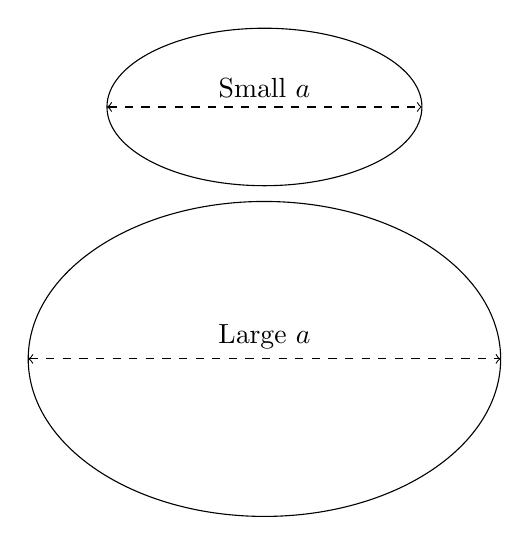
\begin{tikzpicture}[scale=1]
						\pgfmathsetmacro{\o}{1.6}
						\draw (0,\o) ellipse (2 and 1);
						\draw [<->, dashed] (-2,\o) -- (2,\o);
						\node at (0,\o) [anchor=south] {Small \( a \)};

						\draw (0,-\o) ellipse (3 and 2);
						\draw [<->, dashed] (-3,-\o) -- (3,-\o);
						\node at (0,-\o) [anchor=south] {Large \( a \)};
					\end{tikzpicture}
				\end{center}
				\caption{Small and large semi-major axes.}
				\label{figA}
			\end{figure}

			The second orbital element, \( e \), is the eccentricity of the orbit. This is useful in determining the aspect ratio of the orbit, or how ``squished'' an elliptical orbit is. Additionally, it is also the eccentricity of the ellipse created by the orbit as demonstrated in Fig.~\ref{figB}.

			\begin{figure}[hbtp]
				\begin{center}
					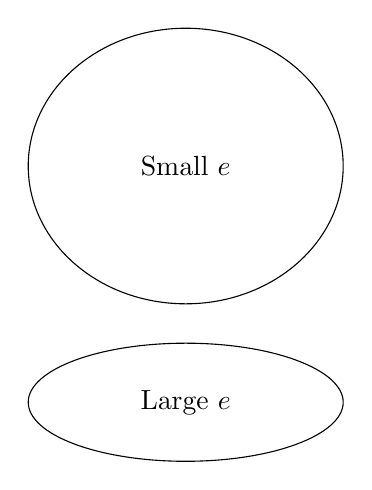
\begin{tikzpicture}[scale=1]
						\pgfmathsetmacro{\o}{1.5}
						\draw (0,\o) ellipse (2 and 1.75);
						\node at (0,\o) [anchor=center] {Small \( e \)};

						\draw (0,-\o) ellipse (2 and 0.75);
						\node at (0,-\o) [anchor=center] {Large \( e \)};
					\end{tikzpicture}
				\end{center}
				\caption{Small and large eccentricities.}
				\label{figB}
			\end{figure}

			The third orbital element, \( i \), is the inclination of the orbit. This is useful in determining the tilt of the orbit from the celestial equatorial plane as demonstrated in Fig.~\ref{figC}.

			\begin{figure}[hbtp]
				\begin{center}
					\tdplotsetmaincoords{80}{180}
					\begin{tikzpicture}[tdplot_main_coords, scale=2]
						\pgfmathsetmacro{\o}{1.5}
						\coordinate (O) at (0,0,0);
						\tdplotsetrotatedcoords{0}{15}{0}
						\tdplotdrawarc[color=black, fill=black, opacity=0.1, dashed]{(O)}{1}{0}{360}{anchor=north west, opacity=0.5}{Celestial Equator}
						\tdplotdrawarc[tdplot_rotated_coords, color=red, fill=red, opacity=0.1]{(O)}{1}{0}{360}{anchor=south west, opacity=0.5}{Orbital Plane}
						\tdplotsetrotatedcoords{90}{90}{90}
						\tdplotdrawarc[tdplot_rotated_coords, color=blue, ->]{(O)}{1}{0}{15}{anchor=west}{Small \( i \)}
					\end{tikzpicture}

					\tdplotsetmaincoords{80}{180}
					\begin{tikzpicture}[tdplot_main_coords, scale=2]
						\pgfmathsetmacro{\o}{1.5}
						\coordinate (O) at (0,0,0);
						\tdplotsetrotatedcoords{0}{50}{0}
						\tdplotdrawarc[color=black, fill=black, opacity=0.1, dashed]{(O)}{1}{0}{360}{anchor=north west, opacity=0.5}{Celestial Equator}
						\tdplotdrawarc[tdplot_rotated_coords, color=red, fill=red, opacity=0.1]{(O)}{1}{0}{360}{anchor=south west, opacity=0.5}{Orbital Plane}
						\tdplotsetrotatedcoords{90}{90}{90}
						\tdplotdrawarc[tdplot_rotated_coords, color=blue, ->]{(O)}{1}{0}{50}{anchor=west}{Large \( i \)}
					\end{tikzpicture}
				\end{center}
				\caption{Small and large inclinations.}
				\label{figC}
			\end{figure}

			The fourth orbital element, \( \Omega \), is the RAAN, or the longitude of the AN\@. It is the angle between \( \aries \) and \( \ascnode \) measured as a positive rotation on the celestial equator, or eastward from \( \aries \). This is useful in determining how rotated an orbit is on Earth's equator as demonstrated in Fig.~\ref{figD}. Because the stars and constellations generally don't move appreciably on a human timescale, the standard coordinate system used is based on the position of the stars and is called the celestial coordinate system. The first two planes of importance for celestial mechanics are the celestial equatorial plane, or the plane created by the Earth's equator, and the ecliptic plane, or the plane created by the Earth's orbit around the Sun. For Earth-orbiting satellites, the celestial equatorial plane is always used as the reference plane that the orbital elements are measured off of. Additionally, this system has a reference direction, designated \( \vhat{I} \), in the direction of the vernal equinox or the First Point of Aries, \( \aries \). This direction is determined when the line created by the intersection of the celestial equatorial plane and the ecliptic plane perfectly points toward the gravitational center of the Sun, meaning the Sun is coplanar with both the equatorial plane and the ecliptic plane. Specifically, the \( \aries \) vector points towards the Sun when the Sun appears to move from the Southern Hemisphere towards the Northern Hemisphere. Finally, the last plane of interest for orbital mechanics is the orbital plane, or the plane created by a satellite's orbit around the Earth. The intersection of the orbital plane and the equatorial plane creates a line called the line of nodes. The points at which this line intersects the satellite's orbit are labeled the AN, or \( \ascnode \), and DN, or \( \descnode \). Specifically, the AN is the point when the satellite crosses from below the equatorial plane to above it, and the DN is the point when the satellite crosses from above the equatorial plane to below it.

			\begin{figure}[hbtp]
				\begin{center}
					\tdplotsetmaincoords{65}{30}
					\begin{tikzpicture}[tdplot_main_coords, scale=2]
						\pgfmathsetmacro{\o}{45}
						\coordinate (O) at (0,0,0);
						\tdplotsetrotatedcoords{-\o}{30}{0}
						\tdplotdrawarc[color=Snow4, fill=Snow4, opacity=0.3, dashed]{(O)}{1}{\o}{\o+180}{}{}
						\tdplotdrawarc[tdplot_rotated_coords, color=Pink2, fill=Pink2, opacity=0.5]{(O)}{1}{0}{360}{anchor=south west, color=red, opacity=0.5}{Orbital Plane}
						\tdplotdrawarc[color=Snow4, fill=Snow4, opacity=0.3, dashed]{(O)}{1}{\o+180}{\o+360}{anchor=north, color=black, opacity=0.5}{Celestial Equator}
						\draw [->, dashed] (O) -- (1.25,0,0) node[anchor=north east] {\( \aries \)};
						\tdplotdrawarc[tdplot_rotated_coords, color=red, opacity=0.5, ->]{(O)}{1}{0}{1}{}{}
						\tdplotdrawarc[tdplot_rotated_coords, color=red, opacity=0.5, ->]{(O)}{1}{180}{181}{}{}
						\draw [tdplot_rotated_coords, color=orange, fill=orange, opacity=0.9, dashed] (0,-1,0) node[circle, fill, inner sep=0.01, anchor=center] {.} node[anchor=north east] {\( \descnode \)} -- (0,1,0) node[circle, fill, inner sep=0.01, anchor=center] {.} node[anchor=south west] {\( \ascnode \)};
						\tdplotdrawarc[color=Green4, ->, thick]{(O)}{1}{0}{\o}{anchor=west}{Small \( \Omega \)}
					\end{tikzpicture}

					\tdplotsetmaincoords{65}{30}
					\begin{tikzpicture}[tdplot_main_coords, scale=2]
						\pgfmathsetmacro{\o}{290}
						\coordinate (O) at (0,0,0);
						\tdplotsetrotatedcoords{\o-90}{30}{0}
						\tdplotdrawarc[color=Snow4, fill=Snow4, opacity=0.3, dashed]{(O)}{1}{\o}{\o+180}{}{}
						\tdplotdrawarc[tdplot_rotated_coords, color=Pink2, fill=Pink2, opacity=0.5]{(O)}{1}{0}{360}{}{}
						\node at (1.75, 0, 1) [anchor=south east, color=red, opacity=0.5]{Orbital Plane};
						\node at (1.25, -1, 0) [anchor=north, color=black, opacity=0.5]{Celestial Equator};
						\tdplotdrawarc[color=Snow4, fill=Snow4, opacity=0.3, dashed]{(O)}{1}{\o+180}{\o+360}{}{}
						\draw [->, dashed] (O) -- (1.25,0,0) node[anchor=north east] {\( \aries \)};
						\tdplotdrawarc[tdplot_rotated_coords, color=red, opacity=0.5, ->]{(O)}{1}{0}{1}{}{}
						\tdplotdrawarc[tdplot_rotated_coords, color=red, opacity=0.5, ->]{(O)}{1}{180}{181}{}{}
						\draw [tdplot_rotated_coords, color=orange, fill=orange, opacity=0.9, dashed] (0,-1,0) node[circle, fill, inner sep=0.01, anchor=center] {.} node[anchor=south] {\( \descnode \)} -- (0,1,0) node[circle, fill, inner sep=0.01, anchor=center] {.} node[anchor=north] {\( \ascnode \)};
						\tdplotdrawarc[color=Green4, ->, thick]{(O)}{1}{0}{\o}{anchor=south}{Large \( \Omega \)}
					\end{tikzpicture}
				\end{center}
				\caption{Small and large RAANs.}
				\label{figD}
			\end{figure}

			The fifth orbital element, \( \omega \), is the argument of periapsis. It is the angle between \( \ascnode \) and the periapsis of the orbit, measured in the direction of the path of the orbiting body. This is useful in determining how rotated an orbit is in its orbital plane, with respect to the celestial equator, or the line of nodes, as demonstrated in Fig.~\ref{figE}.

			\begin{figure}[hbtp]
				\begin{center}
					\tdplotsetmaincoords{70}{25}
					\begin{tikzpicture}[tdplot_main_coords, scale=2]
						\pgfmathsetmacro{\o}{15}
						\coordinate (O) at (0,0,0);
						\tdplotsetrotatedcoords{\o-90}{30}{0}
						\tdplotdrawarc[color=Snow4, fill=Snow4, opacity=0.3, dashed]{(O)}{1}{\o}{\o+180}{}{}
						\tdplotdrawarc[tdplot_rotated_coords, color=Pink2, fill=Pink2, opacity=0.5]{(O)}{1}{0}{360}{anchor=north, color=red, opacity=0.5}{Orbital Plane}
						\tdplotdrawarc[color=Snow4, fill=Snow4, opacity=0.3, dashed]{(O)}{1}{\o+180}{\o+360}{}{}
						\node at (-0.3, 0, 0.3) [anchor=north, color=black, opacity=0.5]{Celestial Equator};
						\tdplotdrawarc[tdplot_rotated_coords, color=red, opacity=0.5, ->]{(O)}{1}{45}{46}{}{}
						\tdplotdrawarc[tdplot_rotated_coords, color=red, opacity=0.5, ->]{(O)}{1}{225}{226}{}{}
						\draw [tdplot_rotated_coords, color=orange, fill=orange, opacity=0.9, dashed] (0,-1,0) node[circle, fill, inner sep=0.01, anchor=center] {.} node[anchor=north east] {\( \descnode \)} -- (0,1,0) node[circle, fill, inner sep=0.01, anchor=center] {.} node[anchor=south west] {\( \ascnode \)};
						\tdplotsetrotatedcoords{\o-90}{30}{35}
						\draw [tdplot_rotated_coords, color=Cyan4, fill=Cyan4, opacity=0.9, dashed] (0,-1,0) node[circle, fill, inner sep=0.01, anchor=center] {.} node[anchor=north east] {} -- (0,1,0) node[circle, fill, inner sep=0.01, anchor=center] {.} node[anchor=south west] {Periapsis};
						\tdplotsetrotatedcoords{\o-90}{30}{0}
						\tdplotdrawarc[tdplot_rotated_coords, color=Purple2, ->, thick]{(O)}{1}{90}{125}{anchor=south west}{Small \( \omega \)}
					\end{tikzpicture}

					\tdplotsetmaincoords{70}{25}
					\begin{tikzpicture}[tdplot_main_coords, scale=2]
						\pgfmathsetmacro{\o}{15}
						\coordinate (O) at (0,0,0);
						\tdplotsetrotatedcoords{\o-90}{30}{0}
						\tdplotdrawarc[color=Snow4, fill=Snow4, opacity=0.3, dashed]{(O)}{1}{\o}{\o+180}{}{}
						\tdplotdrawarc[tdplot_rotated_coords, color=Pink2, fill=Pink2, opacity=0.5]{(O)}{1}{0}{360}{anchor=south west, color=red, opacity=0.5}{Orbital Plane}
						\tdplotdrawarc[color=Snow4, fill=Snow4, opacity=0.3, dashed]{(O)}{1}{\o+180}{\o+360}{}{}
						\node at (1.5, -1, -0.1) [anchor=north, color=black, opacity=0.5]{Celestial Equator};
						\tdplotdrawarc[tdplot_rotated_coords, color=red, opacity=0.5, ->]{(O)}{1}{45}{46}{}{}
						\tdplotdrawarc[tdplot_rotated_coords, color=red, opacity=0.5, ->]{(O)}{1}{225}{226}{}{}
						\draw [tdplot_rotated_coords, color=orange, fill=orange, opacity=0.9, dashed] (0,-1,0) node[circle, fill, inner sep=0.01, anchor=center] {.} node[anchor=north east] {\( \descnode \)} -- (0,1,0) node[circle, fill, inner sep=0.01, anchor=center] {.} node[anchor=south west] {\( \ascnode \)};
						\tdplotsetrotatedcoords{\o-90}{30}{260}
						\draw [tdplot_rotated_coords, color=Cyan4, fill=Cyan4, opacity=0.9, dashed] (0,-1,0) node[circle, fill, inner sep=0.01, anchor=center] {.} node[anchor=north east] {} -- (0,1,0) node[circle, fill, inner sep=0.01, anchor=center] {.} node[anchor=north] {Periapsis};
						\tdplotsetrotatedcoords{\o-90}{30}{0}
						\tdplotdrawarc[tdplot_rotated_coords, color=Purple2, ->, thick]{(O)}{1}{90}{350}{}{}
						\node at (0.1, 0.1, 0.8) [anchor=south east, color=Purple2, ->, thick]{Large \( \omega \)};
					\end{tikzpicture}
				\end{center}
				\caption{Small and large arguments of periapsis.}
				\label{figE}
			\end{figure}

			The sixth and final orbital element, \( \nu \), is the true anomaly. It is the angular position of the orbiting body in its orbit measured from the point about which the body orbits, or the focus of the ellipse of the orbit, in the direction of the path of the orbiting body, with respect to its periapsis. This is useful in determining exactly where the orbiting body is in its orbiting path as demonstrated in Fig.~\ref{figF}.

			\begin{figure}[hbtp]
				\begin{center}
					\tdplotsetmaincoords{0}{0}
					\begin{tikzpicture}[tdplot_main_coords, scale=0.95]
						\pgfmathsetmacro{\o}{1.561}
						\draw [color=Pink2, fill=Pink2, opacity=0.5] (-\o,0,0) ellipse (2 and 1.25);
						\tdplotdrawarc[color=red, opacity=0.5, ->]{(-\o,0,0)}{1.25}{90}{91}{}{}
						\tdplotdrawarc[color=red, opacity=0.5, ->]{(-\o,0,0)}{1.25}{270}{271}{}{}
						\draw [color=Cyan4, fill=Cyan4, opacity=0.9, dashed] (-2-\o,0,0) node[circle, fill, inner sep=0.01, anchor=center] {.} node[anchor=north east] {} -- (2-\o,0,0) node[circle, fill, inner sep=0.01, anchor=center] {.} node[anchor=west] {Periapsis};
						\draw [color=red, fill=red, opacity=0.9, dashed] (0,0,0) node[circle, fill, inner sep=0.01, anchor=center] {.} node[anchor=north east] {} -- (0.119,0.678,0) node[circle, fill, inner sep=0.01, anchor=center] {.} node[anchor=south west] {Satellite};
						\tdplotdrawarc[color=red, opacity=0.9, ->, thick]{(0,0,0)}{0.4}{0}{80}{}{}
						\node at (0,0,0) [circle, fill, inner sep=0.01, anchor=center] {.};
						\node at (0,-0.3) [anchor=center] {Barycenter};
						\node at (0.4,0.4,0) [anchor=west, color=red, opacity=0.9] {Small \( \nu \)};
					\end{tikzpicture}

					\tdplotsetmaincoords{0}{0}
					\begin{tikzpicture}[tdplot_main_coords, scale=0.95]
						\pgfmathsetmacro{\o}{01.561}
						\draw [color=Pink2, fill=Pink2, opacity=0.5] (-\o,0,0) ellipse (2 and 1.25);
						\tdplotdrawarc[color=red, opacity=0.5, ->]{(-\o,0,0)}{1.25}{90}{91}{}{}
						\tdplotdrawarc[color=red, opacity=0.5, ->]{(-\o,0,0)}{1.25}{270}{271}{}{}
						\draw [color=Cyan4, fill=Cyan4, opacity=0.9, dashed] (-2-\o,0,0) node[circle, fill, inner sep=0.01, anchor=center] {.} node[anchor=north east] {} -- (2-\o,0,0) node[circle, fill, inner sep=0.01, anchor=center] {.} node[anchor=west] {Periapsis};
						\draw [color=red, fill=red, opacity=0.9, dashed] (0,0,0) node[circle, fill, inner sep=0.01, anchor=center] {.} node[anchor=north east] {} -- (-0.157,-0.89,0) node[circle, fill, inner sep=0.01, anchor=center] {.} node[anchor=north west] {Satellite};
						\tdplotdrawarc[color=red, opacity=0.9, ->, thick]{(0,0,0)}{0.4}{0}{260}{}{}
						\node at (0,0,0) [circle, fill, inner sep=0.01, anchor=center] {.};
						\node at (0,0.6) [anchor=center] {Barycenter};
						\node at (-1.75,-0.5,0) [anchor=west, color=red, opacity=0.9] {Large \( \nu \)};
					\end{tikzpicture}
				\end{center}
				\caption{Small and large true anomalies.}
				\label{figF}
			\end{figure}

		\subsection{Classical Orbital Elements}

			Putting together all six of these classical orbital elements, any orbiting body can be fully described and positioned, as demonstrated in Fig.~\ref{figG}.

			\begin{figure}[hbtp]
				\begin{center}
					\tdplotsetmaincoords{70}{110}
					\begin{tikzpicture}[tdplot_main_coords, scale=3.5]
						\pgfmathsetmacro{\r}{1}
						\pgfmathsetmacro{\O}{45}
						\pgfmathsetmacro{\i}{30}
						\pgfmathsetmacro{\f}{35}
						\coordinate (O) at (0,0,0);
						\tdplotdrawarc[color=Snow4, fill=Snow4, opacity=0.3, dashed]{(O)}{\r}{\O}{180+\O}{}{}
						\draw [->, thick] (O) -- (0,1.2,0) node[anchor=north west] {\( \vhat{J} \)};
						\tdplotsetrotatedcoords{-\O}{\i}{0}
						\node at (0,-\r+0.4,0.4) [left,text width=4em, color=black, opacity=0.5] {Celestial Equator};
						\tdplotdrawarc[tdplot_rotated_coords, color=Pink2, fill=Pink2, opacity=0.5]{(O)}{\r}{0}{360}{}{}
						\tdplotdrawarc[tdplot_rotated_coords, color=red, opacity=0.5, ->]{(O)}{1}{45}{45.1}{}{}
						\tdplotdrawarc[tdplot_rotated_coords, color=red, opacity=0.5, ->]{(O)}{1}{225}{225.1}{}{}
						\draw[tdplot_rotated_coords, color=Cyan4, dashed] (1,0,0) node[circle, fill, inner sep=0.01, anchor=center] {.} -- (0,0,0);
						\tdplotdrawarc[color=Snow4, fill=Snow4, opacity=0.3, dashed]{(O)}{\r}{\O}{-\O-90}{}{}
						\draw [->, thick] (O) -- (2.2,0,0) node[anchor=north east] {\( \aries \)};
						\draw [->, thick] (O) -- (0,0,0.8) node[anchor=south] {\( \vhat{K} \)};
						\tdplotsetrotatedcoords{\O}{0}{0}
						\draw [tdplot_rotated_coords, color=orange, dashed] (-1,0,0) node[circle, fill, inner sep=0.01, anchor=center] {.} node [above left] {\( \descnode \)} -- (1,0,0) node[circle, fill, inner sep=0.01, anchor=center] {.} node [below right] {\( \ascnode \)};
						\tdplotdrawarc[color=Green4, ->, thick]{(O)}{.33*\r}{0}{\O}{anchor=north}{\( \Omega \)}
						\tdplotsetrotatedcoords{-\O}{\i}{0}
						\begin{scope}[tdplot_rotated_coords]
							\draw[->] (O) -- (0,0,1) node [above] {\( \vhat{W} \)};
							\draw[color=Cyan4, dashed] (0,0,0) -- (-1,0,0) node[circle, fill, inner sep=0.01, anchor=center] {.} node [anchor=south] {\( r_p \)};
							\tdplotdrawarc[color=Purple2, ->, thick]{(O)}{.33*\r}{90}{180}{anchor=west}{\( \omega \)}
							\coordinate (P) at (180+\f:\r);
							\draw [color=red] (O) -- (P) node [anchor=south] {\( \vec{r} \)};
							\tdplotdrawarc[color=red, ->, thick]{(O)}{.33*\r}{180}{180+\f}{anchor=south west}{\( \nu \)}
						\end{scope}
						\tdplotsetrotatedcoords{-\O+\f}{\i}{0}
						\tdplotsetrotatedcoordsorigin{(P)}
						\begin{scope}[tdplot_rotated_coords,scale=.2]
							\fill [color=red] (P) circle (.33ex);
						\end{scope}
						\tdplotsetthetaplanecoords{-\f}
						\tdplotdrawarc[tdplot_rotated_coords, color=blue, ->, thick]{(O)}{.7*\r}{0}{\i}{anchor=south}{$i$}
					\end{tikzpicture}
				\end{center}
				\caption{All classical orbital elements.}
				\label{figG}
			\end{figure}

	\section{3D Development in Unity}

		\subsection{Player and Camera Control}
			The camera is controlled by

		\subsection{Parsing TLEs}
			TLEs are 
			The data is extracted by

		\subsection{Initial Desmos Development}
			Desmos' 3D graphing calculator was used to create the initial coordinate axis rotations.
			\begin{equation}
				a+b=\gamma\label{eq}
			\end{equation}
			Equation \eqref{eq} is

		\subsection{Implementation in Unity}
			Using the results from the Desmos experiments, 

	\section{Conclusion}

		\subsection{Project Deliverables}
			The final deliverable for the project is

		\subsection{Challenges and Difficulties}
			Many challenges and difficulties were faced throughout the development of this project.

		\subsection{Thoughts on Project and Future Development}
			For additional development in the future, I would like to add in all of the visual elements that I did not have time to add into this initial release of the project.

	\section*{Usage Information and Notes}
		A TLE is entered in this box

		The camera is moved via

		Clicking the green button labeled \texttt{START}

		Clicking the red button labeled \texttt{STOP PROGRAM}

		The source code for my final project can be found in the GitHub repository for this project: \texttt{LINK}

	\begin{thebibliography}{00}
		\bibitem{b1} G. Eason, B. Noble, and I. N. Sneddon, ``On certain integrals of Lipschitz-Hankel type involving products of Bessel functions,'' Phil. Trans. Roy. Soc. London, vol. A247, pp. 529--551, April 1955.
		\bibitem{b2} J. Clerk Maxwell, A Treatise on Electricity and Magnetism, 3rd ed., vol. 2. Oxford: Clarendon, 1892, pp.68--73.
	\end{thebibliography}
\end{document}